\section{Limits are dangerous}
\label{limits}
Limits should be taken with care. A number of theorems describe 
when we can change order of limits and when we can not, how
we can approach to the limit and all that.

Imagine a bucket with small hall at the bottom (in Ideal world),
so we can say that the hole is so small that for all times the bucket remains practically full.
On the other hand we can say that the bucket will be empty if we wait long enough.

Important fact is that two smooth curve may coincide as sets of points, but have
different lengths. Let $ y_n= \sin(n x)/n $ on the  interval $ 0\le x \le 2 \pi $. 
Calculation of length of sinusoidal curve is a simple exercise in elliptic integrals:
\begin{equation}
   \label {sin-length}
   \begin{split}
       l_n=\int_0^{2 \pi}\sqrt{1+\cos^2(nx)}dx\\
       =\int_0^{2 n \pi}\sqrt{1+\cos^2(z)}dz/n\\
       =\int_0^{2 \pi}\sqrt{1+\cos^2(z)}dz\quad \text{does not depend on n}  \\
       =4 \sqrt{2} \int_0^{\pi/2}\sqrt{1-\frac{1}{2} \sin^2(z)}dz\\
       =4 \sqrt{2} E(\frac{1}{\sqrt{2}}) \approx 1.351
   \end{split}
\end{equation}  
and ratio of its length to that of segment is $ \approx 1.22 $ independent of $ n $.
On the other hand maximal distance between the curve and straight segment $ d_n=1/n $ 
vanishes for $ n\rightarrow \infty $.

Contrary to common belief not every properly set problem in
classical mechanics has unique solution. Let's take for example
a (rigid) beam on three (rigid) pillars (see fig.\ref{beam3}).
\begin{figure}[h]
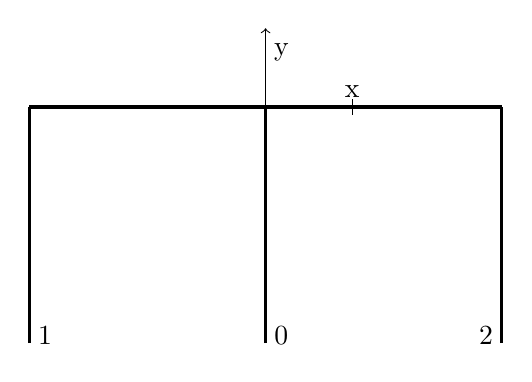
\begin{tikzpicture}
%\draw[thin,dotted] (-3,-3) grid (3,1);
\draw[->] (0,0) -- (0,1);
\node at (0.2,0.7)  {y};
\draw[very thick] (-3,0) -- (3,0);
\draw[very thick] (-3,-3) -- (-3,0);
\draw[very thick] (3,-3) -- (3,0);
\draw[very thick] (0,-3) -- (0,0);
\draw (1.1,-0.1) -- (1.1,0.1);
\node at (1.1,0.2) {x};
\node at (-2.8,-2.9) {1};
\node at (0.2,-2.9) {0};
\node at (2.8,-2.9) {2};
\end{tikzpicture}
\caption{Beam on 3 pillars}
\label {beam3}
\end{figure}
Let the weight of the beam be $W$ and length $2 L$.
Balance of forces gives:
\begin{equation}
        F_0+F_1+F_2=W \label {bf}
\end{equation}
Balance of torques gives:
\begin{equation}
        F_1 L=F_2 L \label {bt}
\end{equation}

   So we have only two equations for three
unknown forces. From the symmetry we can get that $F_1=F_2$. 
(We know that this already from balance of torques.)

{\em First solution}:
All pillars and beam are absolutely rigid. Then
if we pull out the middle pillar nothing will change.
So $F_0=0$ and $F_1=F_2=W/2$.

{\em Second solution}
All pillars and beam are absolutely rigid. Then
we can cat beam at the center and will have two
beams laying on two pillars each.
So $F_0=W/2$ and $F_1=F_2=W/4$.

{\em Third solution}
Beam is absolutely rigid, pillars are very hard springs.
Since beam is horizontal, small change in length is 
equal to all pillars so $F_0=F_1=F_2=w/3$


{\em Fourth solution}
Pillars are rigid, beam is elastic. This case needs
some calculations, well known in elasticity theory
(see e.g \cite {Landau-Lifshitz-7}).
The results is $F_0=5 W/8$ and $F_1=F_2=3 W/16$.

It is clear that all these solutions (and more can be
produced) are limiting cases of standard elasticity 
problem when elasticity coefficients go to infinity.
So generally we can't simply neglect elastic deformations,
we should be more careful.

